\section{Pianificazione}
Nella pianificazione, il responsabile suddividerà il lavoro in attività e le assegnerà a ciascun membro del team qbteam.
Lo scopo è quello di mostrare come verrà svolto il lavoro, valutare i progressi nel progetto e anticipare i problemi che potrebbero sorgere preparando così delle soluzioni a tali problemi. 
La pianificazione di progetto è stata organizzata seguendo le scadenze presenti nella sezione Scadenze.
Lo sviluppo del progetto è stato suddiviso nei seguenti 5 macro periodi: 
\begin{itemize}
	\item Analisi;
	\item Progettazione architetturale;
	\item Progettazione di dettaglio e codifica;
	\item Validazione e collaudo;
\end{itemize}
Ogni macro periodo sarò suddiviso a sua volta in altri periodi più brevi in cui verranno elencate le diverse attività che il gruppo qbteam svolgerà.


\subsection{Analisi}

\subsubsection{Periodo 1} 
Dal al\\
\begin{itemize}
	\item \textbf{};
	\item \textbf{};
	\item \textbf{};
	\item \textbf{};
\end{itemize}
\subsubsection{Periodo 2} 
Dal al
\begin{itemize}
	\item \textbf{};
	\item \textbf{};
	\item \textbf{};
	\item \textbf{};
\end{itemize}
\subsubsection{Periodo 3} 
Dal 2019-01-14 al 2019-01-20
\begin{itemize}
	\item \textbf{};
	\item \textbf{};
	\item \textbf{};
	\item \textbf{};
\end{itemize}
\subsubsection{Diagramma di Gantt delle attività}
\begin{figure}[h]
	\includegraphics[scale=0.45]{sezioni/DiagrammiGantt/  }
	\caption{Diagramma di Gantt delle attività di Analisi}
\end{figure}


\subsection{Progettazione architetturale}
Periodo: dal 2019-01-22 al 2019-03-15.
\\Inizia al termine dell'Analisi dei Requisiti e finisce con la data di consegna della Revisione di Progettazione.
\\In questo macro periodo viene definita una soluzione architetturale in modo da soddisfare i requisiti individuati nel periodo di Analisi dei Requisiti.

\subsubsection{Periodo 1} 
Dal 2019-01-22 al 2019-02-17
\begin{itemize}
	\item \textbf{Normazione:} aggiornamento delle norme;
	\item \textbf{Analisi dei requisiti:} aggiornamento dell'analisi dei requisiti;
	\item \textbf{Pianificazione:} aggiornamento della pianificazione;
	\item \textbf{Gestione qualità:} aggiornamento dei metodi sulla qualità;
	\item \textbf{Approfondimento sulle tecnologie:} aggiornamento delle tecnologie che si dovranno utilizzare;
	\item \textbf{Verifica};
\end{itemize}
\subsubsection{Periodo 2} 
Dal 2019-02-18 al 2019-03-08
\begin{itemize}
	\item \textbf{Studio delle tecnologie:} IAAS Kubernetes\ap{G} o PaaS\ap{G}, Openshift\ap{G} o Rancher\ap{G}, LDAP\ap{G} e GPS\ap{G};
	\item \textbf{Tecnology Baseline\ap{G}:} redazione della tecnology baseline;
	\item \textbf{Proof of Concept\ap{G}:} rappresentazione della Baseline\ap{G};
	\item \textbf{Codifica:} viene codificato il Proof of Concept;
\end{itemize}
\subsubsection{Periodo 3} 
Dal 2019-03-09 al 2019-03-15
\begin{itemize}
	\item \textbf{Preparazione per la revisione di avanzamento};
\end{itemize}
\subsubsection{Diagramma di Gantt delle attività}
\begin{figure}[h]
	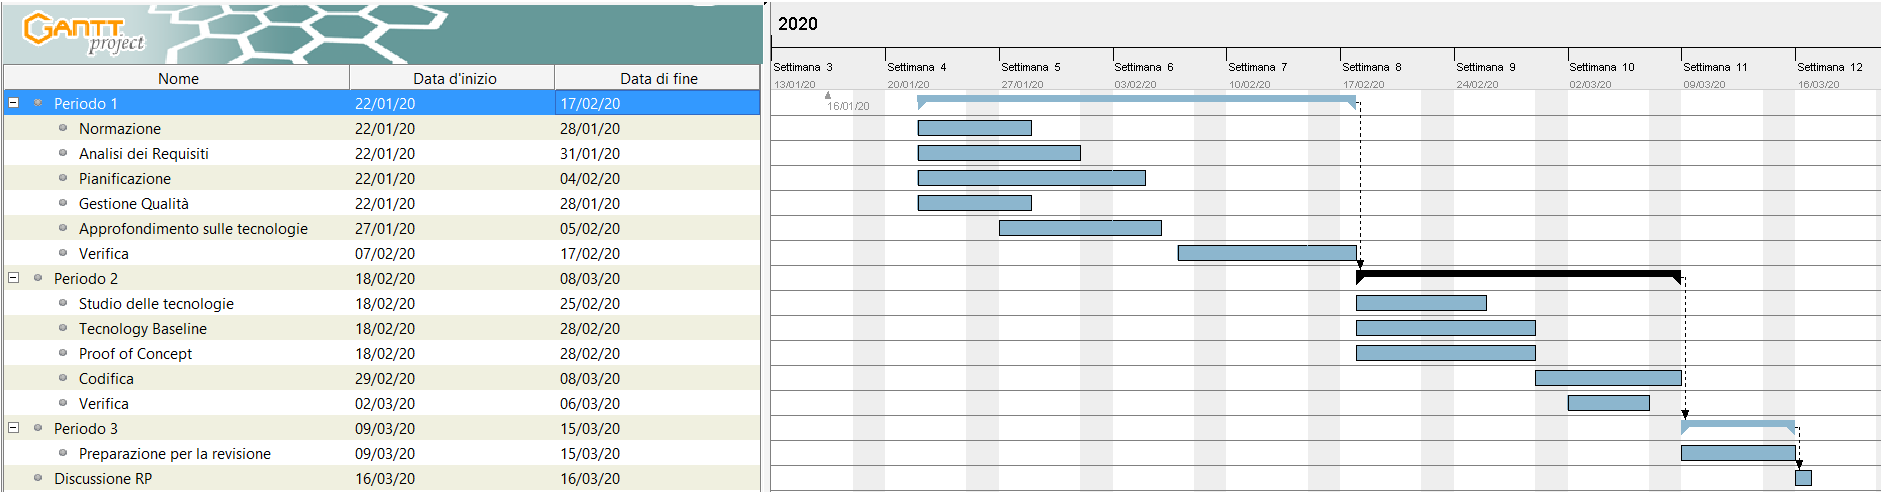
\includegraphics[scale=0.45]{sezioni/DiagrammiGantt/RP.png}
	\caption{Diagramma di Gantt delle attività di Progettazione architetturale}
\end{figure}

\subsection{Progettazione di dettaglio e codifica}

\subsubsection{Periodo 1} 
Dal al
\begin{itemize}
	\item \textbf{};
	\item \textbf{};
	\item \textbf{};
	\item \textbf{};
\end{itemize}
\subsubsection{Periodo 2} 
Dal al
\begin{itemize}
	\item \textbf{};
	\item \textbf{};
	\item \textbf{};
	\item \textbf{};
\end{itemize}
\subsubsection{Periodo 3} 
Dal 2019-04-13 al 2019-04-19
\begin{itemize}
	\item \textbf{};
	\item \textbf{};
	\item \textbf{};
	\item \textbf{};
\end{itemize}
\subsubsection{Diagramma di Gantt delle attività}
\begin{figure}[h]
	\includegraphics[scale=0.45]{sezioni/DiagrammiGantt/ }
	\caption{Diagramma di Gantt delle attività di Progettazione di dettaglio e codifica}
\end{figure}


\subsection{Validazione e collaudo}

\subsubsection{Periodo 1} 
Dal al
\begin{itemize}
	\item \textbf{};
	\item \textbf{};
	\item \textbf{};
	\item \textbf{};
\end{itemize}
\subsubsection{Periodo 2} 
Dal al
\begin{itemize}
	\item \textbf{};
	\item \textbf{};
	\item \textbf{};
	\item \textbf{};
\end{itemize}
\subsubsection{Periodo 3} 
Dal 2019-05-11 al 2019-05-17
\begin{itemize}
	\item \textbf{};
	\item \textbf{};
	\item \textbf{};
	\item \textbf{};
\end{itemize}
\subsubsection{Diagramma di Gantt delle attività}
\begin{figure}[h]
	\includegraphics[scale=0.45]{sezioni/DiagrammiGantt/ }
	\caption{Diagramma di Gantt delle attività di Validazione e Collaudo}
\end{figure}
